% !TEX program = pdflatex
\documentclass[10pt,a4paper]{article}

% -----------------------
% Encoding + language
% -----------------------
\usepackage[T1]{fontenc}
\usepackage[utf8]{inputenc}
\usepackage[english]{babel}

% -----------------------
% Scalable fonts (fixes pdfTeX microtype expansion issues)
% -----------------------
\usepackage{lmodern}

% -----------------------
% Typography (safe microtype config)
% -----------------------
\usepackage[final]{microtype}
% If your setup still complains, uncomment the next line:
% \microtypesetup{expansion=false}

% -----------------------
% Page layout
% -----------------------
\usepackage{geometry}
\geometry{margin=1.8cm}
\usepackage{subcaption}

\usepackage{setspace}
\onehalfspacing

% -----------------------
% Math + symbols
% -----------------------
\usepackage{amsmath,amssymb}

% -----------------------
% Figures + tables
% -----------------------
\usepackage{graphicx}
\usepackage{float}
\usepackage{booktabs}

% -----------------------
% Links
% -----------------------
\usepackage[hidelinks]{hyperref}

% -----------------------
% Code listings (optional)
% -----------------------
\usepackage{xcolor}
\usepackage{listings}
\lstset{
  basicstyle=\ttfamily\small,
  breaklines=true,
  frame=single,
  columns=fullflexible,
  showstringspaces=false
}

% -----------------------
% Nice lists
% -----------------------
\usepackage{enumitem}
\setlist{noitemsep, topsep=0.3em}

% -----------------------
% Pipeline Visualisation
% -----------------------
\usepackage{tikz}
\usetikzlibrary{arrows.meta, positioning}

% -----------------------
% Code Visualisation
% -----------------------
\lstset{
  basicstyle=\ttfamily\small,
  breaklines=true,
  frame=single,
  columns=fullflexible,
  showstringspaces=false
}

% -----------------------
% Title meta
% -----------------------
\title{Radar Visualization Pipeline Report}
\author{Aiysha Mei Frutiger, Sandro Barbazza, Senanur Ates,  \\ University of Basel \\ Computer Architecture}
\date{January 19, 2026}

\begin{document}
\maketitle

\begin{abstract}

We built a simple ultrasonic ``radar-style'' scanner that measures distance and visualizes the results live in 2D. An Arduino triggers a URM37 ultrasonic sensor, measures the echo pulse width, converts it to centimeters, and sends one newline-terminated record per sample in the format \texttt{angle,cm}. A servo sweeps the sensor so that each reading becomes an \textit{(angle, distance)} pair that can be drawn in polar coordinates on the host.

The system works reliably for typical indoor test objects: stationary targets produce consistent detections across multiple sweeps, and missing or out-of-range echoes are sent as \texttt{-1} and do not create false points in the visualization. The angular resolution is determined by the sweep step size (2$^\circ$), and the host visualization maintains a bounded state by storing only the latest measurement per angle bucket. Overall, the project demonstrates an end-to-end pipeline from ultrasonic time-of-flight measurement on an Arduino to a real-time radar-style visualization on a computer.
\end{abstract}

\newpage

\begingroup
\renewcommand{\contentsname}{}%
\tableofcontents
\endgroup

\newpage

% ==========================================================
\section{Introduction}
Radar-style visualizations are intuitive and interesting because they make an otherwise invisible measurement process directly observable. This project uses an ultrasonic sensor as a simple stand-in for a radar system: instead of radio waves, we measure ultrasonic time-of-flight and display the result as a scan over angle.

The main motivation is educational. The setup is simple enough to understand end-to-end, but still rich enough to expose core elements of an embedded system and the computer architecture stack around it: timing-based sensing on a microcontroller, embedded processing, serial communication over USB, OS-level device access, and host-side real-time rendering. This allowed us to focus on implementation details and integration issues without the complexity of a full radar system.

Our scope is a complete pipeline from sensor measurements to a live 2D visualization. A servo sweep provides angular sampling so that each reading becomes an \textit{(angle, distance)} observation, which the host can render in polar coordinates.

\paragraph{Contributions.}
\begin{itemize}
  \item End-to-end ultrasonic scan pipeline from time-of-flight echo to live 2D visualization.
  \item Arduino firmware for servo sweep, echo-to-distance conversion, and a newline-framed serial protocol.
  \item Processing-based visualization with robust line parsing and bucket-based refresh behavior.
\end{itemize}

% ==========================================================
\section{Methodology}

\subsection{System-level approach}

We use a simple text-based protocol (\texttt{angle,cm} per line) to keep debugging and integration straightforward across hardware and software. Newline framing defines clear message boundaries on top of the raw serial byte stream.

The Arduino coordinates sensing and actuation, converts echo timing into distance values, and streams the measurements over USB serial. The host reads the resulting serial device, parses the stream into \textit{(angle, distance)} samples, and renders a live 2D radar visualization.

\paragraph{Pipeline.}
\begin{center}
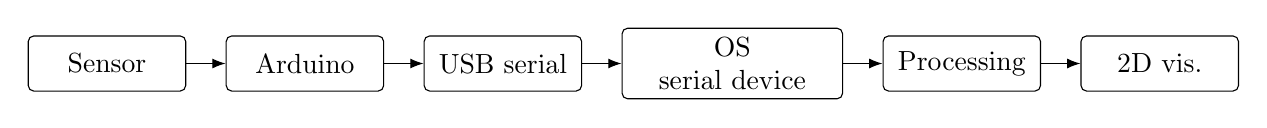
\begin{tikzpicture}[
  box/.style={draw, rounded corners=2pt, minimum height=7mm, minimum width=20mm, align=center},
  arr/.style={-Latex}
]
\node[box] (s) {Sensor};
\node[box, right=5mm of s] (a) {Arduino};
\node[box, right=5mm of a] (u) {USB serial};
\node[box, right=5mm of u, minimum width=28mm] (os) {OS\\serial device};
\node[box, right=5mm of os] (p) {Processing};
\node[box, right=5mm of p] (v) {2D vis.};

\draw[arr] (s) -- (a);
\draw[arr] (a) -- (u);
\draw[arr] (u) -- (os);
\draw[arr] (os) -- (p);
\draw[arr] (p) -- (v);
\end{tikzpicture}
\end{center}

% ==========================================================
\section{Implementation}

\subsection{Hardware}

\paragraph{Bill of materials.}
Arduino Uno Rev3, URM37 ultrasonic sensor, SG90 micro servo, breadboard and jumper wires, external 5\,V / 2\,A supply, and decoupling capacitors (470\,$\mu$F, 100\,nF). The total hardware cost was approximately CHF 98.50 (excluding shipping).

\paragraph{Power and decoupling.}
The Arduino is connected to the host via USB for programming and serial communication. The SG90 servo is powered from the external 5\,V / 2\,A supply to avoid brownouts on the Arduino's 5\,V rail during movement. All grounds (Arduino, sensor, and external supply) are connected to a common ground.

For decoupling, we placed the 470\,$\mu$F electrolytic capacitor directly across the servo supply pins (5\,V to GND) close to the servo connector to buffer short current spikes during movement. In addition, a 100\,nF ceramic capacitor is placed across the URM37 supply pins close to the sensor to filter high-frequency noise on the sensor's power rail.

\paragraph{Pin connections.}
\begin{itemize}
  \item URM37 \texttt{ECHO} (Pin 4) $\rightarrow$ Arduino \texttt{D3} (\texttt{URECHO})
  \item URM37 \texttt{COMP/TRIG} (Pin 6) $\rightarrow$ Arduino \texttt{D5} (\texttt{URTRIG})
  \item SG90 servo signal $\rightarrow$ Arduino \texttt{D9} (\texttt{SERVO\_PIN})
  \item URM37 \texttt{VCC} $\rightarrow$ Arduino \texttt{5V}, \quad URM37 \texttt{GND} $\rightarrow$ Arduino \texttt{GND}
  \item SG90 servo \texttt{VCC} $\rightarrow$ external \texttt{5V}, \quad SG90 servo \texttt{GND} $\rightarrow$ common \texttt{GND}
\end{itemize}

\medskip
\noindent The URM37 sensor is mounted on a self-made servo bracket such that the sweep plane remains stable during scanning.

\subsection{Servo sweep control}

Sweeping is implemented with \texttt{Servo.h}. The servo moves from \texttt{MIN\_ANGLE} to \texttt{MAX\_ANGLE} in
steps of \texttt{STEP\_ANGLE} and then reverses back.

\paragraph{Parameters.}
\texttt{MIN\_ANGLE=10}, \texttt{MAX\_ANGLE=170}, \texttt{STEP\_ANGLE=2}, \texttt{SERVO\_SETTLE\_MS=30 ms},
\texttt{BETWEEN\_READ\_MS=10 ms}. A settling delay is used before each measurement to reduce motion-related errors.

\paragraph{Angle range.}
Although the visualization supports $0^\circ$--$180^\circ$, we scan only $10^\circ$--$170^\circ$. The extreme end positions are mechanically less stable on the SG90/bracket, so restricting the sweep avoids end-stop effects, yields more consistent measurements, and reduces stress on the servo.


\subsection{Measurement and serial protocol}

The ultrasonic sensor returns an \emph{echo pulse width} proportional to time-of-flight. The Arduino triggers the sensor, measures the echo duration (e.g., with \texttt{pulseIn}), converts it to a distance in centimeters, and sends one newline-terminated ASCII record per measurement \texttt{angle,cm}.

Distance is derived from the URM37 echo pulse width $t$ (in $\mu$s) using:
\[
\text{cm} = \frac{t}{50}.
\]
If \texttt{pulseIn} times out (, $t \ge 60000\,\mu\text{s}$) or the measured pulse width exceeds a threshold (, $t \ge 50000\,\mu\text{s}$), the firmware outputs \texttt{-1}.
Serial runs at \texttt{9600} baud and sends one record per sample as \verb|angle,cm\n|.


\subsection{Host-side data flow}

Over USB this data is exposed by the OS as a serial device, which Processing reads as a byte stream, frames into lines, parses angle and distance, and uses to update the visualization state.
On Arduino boards, opening the serial port can reset the microcontroller; therefore the Processing sketch ignores initial startup lines until valid \texttt{angle,cm} records are received.

\paragraph{Pipeline.}
\begin{center}
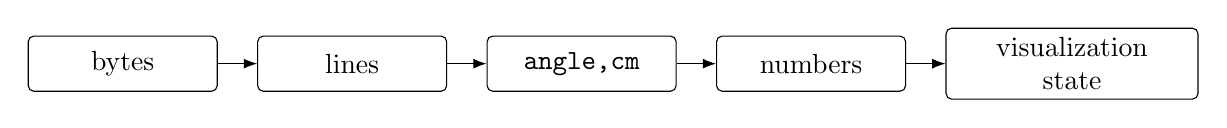
\begin{tikzpicture}[
  box/.style={draw, rounded corners=2pt, minimum height=7mm, minimum width=24mm, align=center},
  arr/.style={-Latex}
]
\node[box] (b) {bytes};
\node[box, right=5mm of b] (l) {lines};
\node[box, right=5mm of l] (t) {\texttt{angle,cm}};
\node[box, right=5mm of t] (n) {numbers};
\node[box, right=5mm of n, minimum width=32mm] (st) {visualization\\state};

\draw[arr] (b) -- (l);
\draw[arr] (l) -- (t);
\draw[arr] (t) -- (n);
\draw[arr] (n) -- (st);
\end{tikzpicture}
\end{center}

\subsection{Visualization}

The visualization renders a radar-style display over $0^\circ$--$180^\circ$, but the measured sweep covers only $10^\circ$--$170^\circ$ to avoid end-stop effects. A sweep line indicates the current angle, and each incoming $(\textit{angle}, \textit{distance})$ measurement is mapped to polar coordinates to draw a point at the corresponding radius. A static grid (concentric arcs and radial lines) provides scale and orientation.

\subsection{Constraints and iterations}

During early development, the hardware prototype did not yet provide a reliable real angle because the servo was not available. To still build and test the full visualization pipeline, we implemented a simulated sweep angle on the host side that increments from $10^\circ$ to $170^\circ$ and back. Once the Arduino started sending \texttt{angle,cm} records, the Processing sketch automatically switched from simulated angles to real angles from the serial stream.

On the mechanical side, the delivered servo bracket did not fit our intended mounting. We therefore built a custom bracket to mount the URM37 securely and maintain a stable sweep plane.

\subsection{Implementation path}

We first prototyped the UI in C using \texttt{raylib}, but the end-to-end system was unstable on Windows due to low-level serial I/O issues (port selection, reset timing, partial lines, contention). We therefore switched to Processing to simplify serial handling using its line-based, event-driven serial library and to iterate faster.

\subsection{Serial parsing and ``bucket'' state}

Processing receives a continuous byte stream and frames it into newline-terminated records. Each line is trimmed, split by comma, and parsed into numeric \textit{angle} and \textit{distance} values; invalid readings are encoded as \texttt{-1} (no detection).

To keep memory bounded and emulate radar refresh behavior, the scan is discretized into fixed-width angle buckets (e.g., \texttt{ANGLE\_BUCKET\_DEG}). Each bucket stores the most recent distance for its slice and is overwritten on the next sweep; a \texttt{-1} clears the corresponding bucket.

Malformed lines (wrong token count or non-numeric values) are ignored. A typical setting is \texttt{ANGLE\_BUCKET\_DEG=2} to match the servo
step size; each bucket stores the latest distance for its angle slice and is overwritten on rescan.



\subsection{Reproducibility notes}

To reproduce the project, flash the Arduino firmware using Arduino IDE 2.3.7 and connect the board via USB. Open the Arduino Serial Monitor at \texttt{9600} baud to verify that the device outputs newline-terminated ASCII records in the form \texttt{angle,cm}, where \texttt{angle} is in $[10,170]$ and \texttt{cm} is either a non-negative distance in centimeters or \texttt{-1} for invalid/out-of-range measurements.

Start the Processing sketch (Processing 4.5.1) and select the correct serial device from \texttt{Serial.list()}. Open the port at \texttt{9600} baud. The sketch ignores startup noise (Arduino reset on port open) until it receives valid \texttt{angle,cm} lines; once valid records arrive, the visualization updates continuously while the servo sweeps.

The expected behavior is a stable sweep over $10^\circ$--$170^\circ$ with detections appearing at consistent angles for stationary objects and disappearing when \texttt{-1} is received for that angle bucket.

% ==========================================================
\section{Evaluation}

\subsection{Functional validation}

We validated the system incrementally. First, we verified the SG90 servo motion using fixed target angles (0$^\circ$, 90$^\circ$, 180$^\circ$). Second, we validated the URM37 distance measurement in isolation by reading the echo pulse width via \texttt{pulseIn} and converting it to centimeters. Third, we combined servo sweep and distance sensing and streamed \texttt{angle,cm} records over serial to test the end-to-end data path. Finally, we switched to explicit sensor triggering (TRIG/ECHO mode) to control measurement timing and handle missing/out-of-range echoes robustly.


\subsection{Performance and limitations}

The angular resolution is set by the sweep step size (\texttt{STEP\_ANGLE=2}$^\circ$), while the refresh rate depends on the servo settling time and the delay between readings (\texttt{SERVO\_SETTLE\_MS=30\,ms}, \texttt{BETWEEN\_READ\_MS=10\,ms}). Measurement stability varies with reflectivity, geometry, and orientation; for example, curved or highly reflective objects such as a stainless-steel water bottle produced less stable readings. Very short distances were occasionally unreliable. We did not notice angle jitter from mechanical play, but we did not quantify it.



\subsection{Match with project goals}

The final system meets the project goal of a compact radar-style scanner that converts ultrasonic time-of-flight into a live 2D visualization. It provides an explainable end-to-end pipeline from embedded measurement on the Arduino to host-side parsing and rendering, and it remains usable both in prototype mode (simulated sweep) and in the final mode with real servo angles. Remaining improvements would focus on calibration and filtering to further stabilize readings and on making the setup more self-contained (e.g., an integrated display and basic calibration routines).

% ==========================================================
\section{Conclusion}

We built an end-to-end ultrasonic ``radar-style'' system that converts echo time-of-flight into a live 2D visualization. The stack is observable from Arduino-side signal timing and distance conversion, through USB serial transport, to host-side parsing and rendering in Processing.

A main takeaway was that end-to-end reliability depends on small integration details across layers. On the communication side, newline-framed records and defensive parsing were essential to handle Arduino reset noise, partial reads, and invalid measurements without producing false points. On the hardware side, stable power delivery, decoupling, and a mechanically rigid sensor mount were equally important to obtain consistent measurements during the sweep.

A further lesson was how to communicate with an Arduino from a higher-level host program over USB serial, and how to interpret the incoming data stream and use it meaningfully inside an application.

Overall, the project achieved a working and explainable sensing-to-visualization pipeline and clarified how embedded measurements can be robustly streamed and interpreted by a higher-level host application.


\paragraph{Self-assessment and outlook.}

We intentionally kept the system small to understand each part of the pipeline. With more time, we would improve measurement stability (e.g., filtering and more robust handling of very short distances) and add a simple calibration routine for sweep limits and sensor offset. A further extension would be an on-device display and basic controls to reduce dependence on the PC.

\paragraph{Division of labor.}

All group members assembled the hardware setup and testing. Sandro implemented the main Arduino sensing/communication code and built the stand/chassis. Senanur developed the Arduino servo sweep control. Aiysha implemented the Processing visualization, including parsing and bucket-based rendering.

% ==========================================================
\newpage
\section*{References}
\addcontentsline{toc}{section}{References}

\begin{itemize}
  \item Processing (project homepage + downloads): \\\url{https://processing.org/} \url{https://processing.org/download/} % :contentReference[oaicite:0]{index=0}
  \item Processing Serial library reference (Serial class): \\\url{https://processing.org/reference/libraries/serial/Serial.html} % :contentReference[oaicite:1]{index=1}
  \item Processing Serial library reference (bufferUntil): \\\url{https://processing.org/reference/libraries/serial/Serial_bufferUntil_.html} % :contentReference[oaicite:2]{index=2}
  \item Processing Serial library reference (readStringUntil — common alternative used with newline framing): \\\url{https://processing.org/reference/libraries/serial/Serial_readStringUntil_.html} % :contentReference[oaicite:3]{index=3}
  \item Processing Serial library reference (serialEvent): \\\url{https://processing.org/reference/libraries/serial/Serial_serialEvent_.html} % :contentReference[oaicite:4]{index=4}
  \item Arduino servo library:\\
  \url{https://docs.arduino.cc/libraries/servo/}
  \item Project source code repository: \\\url{https://github.com/ateschsena/Radar.git}
  \item URM37 Datasheet:\\
  \url{http://www.farnell.com/datasheets/4376735.pdf}
  \item Shop: Farnell - URM37\\
  \url{https://de.farnell.com/}
  \item Shop: Brack - Arduino Uno Rev3/USB-Cable/Breadboard/\\
  \url{https://www.brack.ch/}
  \item Shop: Funduinoshop - Cables\\
  \url{https://funduinoshop.com/}
  \item Shop: Conrad - Condensators/Power supply\\
  \url{https://www.conrad.ch/}
  \item Shop: Shopofthings - Servo SG90/Servo Mount\\
  \url{https://shopofthings.ch/}
\end{itemize}

%==========================================================
\section*{Declaration of Authorship}
\addcontentsline{toc}{section}{Declaration of Authorship}

ChatGPT was used solely to improve the clarity and coherence of the report's language. All ideas, analyses, 
and interpretations presented reflect the group's own work and research.

\newpage

\section*{Appendix}
\addcontentsline{toc}{section}{Appendix}

\begin{lstlisting}[language=C++, caption={Arduino sketch: radar sweep control and serial output (angle,cm)},label={lst:arduino-radar}]

#include <Servo.h>

// =======================
// PIN CONFIGURATION
// =======================
const int SERVO_PIN = 9;   // Servo signal pin
const int URTRIG    = 5;   // Arduino D5 -> URM37 Pin 6 COMP/TRIG
const int URECHO    = 3;   // Arduino D3 -> URM37 Pin 4 ECHO

// =======================
// OBJECTS & VARIABLES
// =======================
Servo radarServo;

// Adjust these if you want different scan behavior
const int MIN_ANGLE = 10;
const int MAX_ANGLE = 170;
const int STEP_ANGLE = 2;

const int SERVO_SETTLE_MS = 30;   // time to let servo reach the angle
const int BETWEEN_READ_MS = 10;   // small gap between trigger and read (optional)

// =======================
// SETUP
// =======================
void setup() {
  radarServo.attach(SERVO_PIN);

  pinMode(URTRIG, OUTPUT);
  pinMode(URECHO, INPUT);

  // URM37 idle state: HIGH
  digitalWrite(URTRIG, HIGH);

  Serial.begin(9600);
  delay(500);

  Serial.println("RADAR SYSTEM READY (URM37 mode)");
  Serial.println("Output format: angle,cm  (cm = -1 means out of range/no pulse)");
}

// =======================
// MAIN LOOP
// =======================
void loop() {
  // Sweep forward
  for (int angle = MIN_ANGLE; angle <= MAX_ANGLE; angle += STEP_ANGLE) {
    scanStep(angle);
  }

  // Sweep backward
  for (int angle = MAX_ANGLE; angle >= MIN_ANGLE; angle -= STEP_ANGLE) {
    scanStep(angle);
  }
}

// =======================
// ONE SCAN STEP
// =======================
void scanStep(int angle) {
  radarServo.write(angle);
  delay(SERVO_SETTLE_MS);

  int cm = measureDistanceURM37();

  // Print as "angle,cm" (easy to parse in Serial Plotter / Processing)
  Serial.print(angle);
  Serial.print(",");
  Serial.println(cm);

  delay(BETWEEN_READ_MS);
}

// =======================
// DISTANCE MEASUREMENT (URM37-style)
// - Trigger: short LOW pulse, then HIGH
// - Echo: LOW-level pulse width
// - Conversion: 50 us = 1 cm  => cm = t / 50
// =======================
int measureDistanceURM37() {
  // Start measurement: short LOW pulse
  digitalWrite(URTRIG, LOW);
  delayMicroseconds(50);
  digitalWrite(URTRIG, HIGH);

  // Read LOW pulse width (timeout 60ms)
  unsigned long t = pulseIn(URECHO, LOW, 60000UL);

  if (t == 0) {
    // no pulse -> out of range / wiring / wrong mode
    return -1;
  }

  // Some example codes treat very large values as invalid
  if (t >= 50000UL) {
    return -1;
  }

  // Convert to cm (integer)
  int cm = (int)(t / 50UL);

  // Optional sanity clamp
  if (cm <= 0 || cm > 500) return -1;

  return cm;
}
\end{lstlisting}

\newpage

\begin{lstlisting}[language=C++, caption={Sensor-only validation: URM37 echo timing and cm conversion},label={lst:urm37-test}]

int URECHO = 3;   // Arduino D3 -> URM37 Pin 4 ECHO
int URTRIG = 5;   // Arduino D5 -> URM37 Pin 6 COMP/TRIG

void setup() {
  Serial.begin(9600);
  pinMode(URTRIG, OUTPUT);
  digitalWrite(URTRIG, HIGH);
  pinMode(URECHO, INPUT);
  delay(500);
  Serial.println("Init");
}

void loop() {
  // Trigger: kurzer LOW-Puls startet Messung
  digitalWrite(URTRIG, LOW);
  delayMicroseconds(50);
  digitalWrite(URTRIG, HIGH);

  unsigned long t = pulseIn(URECHO, LOW, 60000UL); // low-level pulse
  if (t == 0) {
    Serial.println("0 (kein Puls -> wiring/mode)");
  } else if (t >= 50000) {
    Serial.println("Invalid");
  } else {
    Serial.print("cm=");
    Serial.println(t / 50); // 50us = 1cm
  }

  delay(200);
}
\end{lstlisting}

\newpage

\begin{lstlisting}[language=Java, caption={Processing radar visualization (serial parsing + bucket-based refresh)},label={lst:processing-radar}]

import processing.serial.*;

// ====== CONFIG (easy to change) ======
int BAUD = 9600;

// If you're still sending only "distance", UI simulates sweep:
boolean SIMULATE_ANGLE_IF_MISSING = true;
int SIM_ANGLE_MIN = 0;
int SIM_ANGLE_MAX = 180;
float SIM_ANGLE_STEP = 1;      // degrees per frame/update

// Distance mapping:
float MAX_CM = 100;            // scale radar to 0..MAX_CM cm
float RADIUS_PX = 330;         // size of radar on screen

// ===== Persistence (dot stays until overwritten, but fades over time) =====
int ANGLE_BUCKET_DEG = 2;      // 1 = every degree, 2 = less noisy
int MIN_ALPHA = 120;           // never fade below this (0..255)
int FADE_MS = 2000;            // time until dot reaches MIN_ALPHA (ms)

// ====== state ======
Serial port;
float angleDeg = 0;
float distanceCm = -1;

float simAngle = 0;
float simDir = 1;

// Stores one dot per angle bucket
Ping[] latest = new Ping[181];

// Each stored dot remembers: angle bucket, distance, and when it was last updated
class Ping {
  float a, d;
  int bornMs;
  Ping(float a, float d, int bornMs) { this.a = a; this.d = d; this.bornMs = bornMs; }
}

void setup() {
  size(900, 520);
  smooth();
  frameRate(60);

  println("Available serial ports:");
  printArray(Serial.list());

  port = new Serial(this, "COM7", BAUD); // replace with your Arduino COM
  port.bufferUntil('\n'); // read line-by-line

  angleDeg = 0;
  simAngle = 0;
}

void draw() {
  background(0);

  // Simulated sweep if we don't receive angle from serial
  if (SIMULATE_ANGLE_IF_MISSING) {
    simAngle += simDir * SIM_ANGLE_STEP;

    if (simAngle >= SIM_ANGLE_MAX) { simAngle = SIM_ANGLE_MAX; simDir = -1; }
    if (simAngle <= SIM_ANGLE_MIN) { simAngle = SIM_ANGLE_MIN; simDir =  1; }

    if (!lastLineHadAngle) angleDeg = simAngle;
  }

  // Radar origin
  float cx = width * 0.5;
  float cy = height * 0.92;

  drawGrid(cx, cy);
  drawSweepAndUpdateBucket(cx, cy, angleDeg);  // <-- sweep overwrites bucket every time
  drawPersistentDots(cx, cy);

  // UI text
  textAlign(LEFT, TOP);

  fill(0, 255, 0);
  textSize(16);
  text("Angle: " + int(angleDeg) + "°", 20, 30);
  text("Distance: " + int(distanceCm) + " cm", 20, 55);
  text("Mode: " + (lastLineHadAngle ? "REAL angle from Serial" : "SIMULATED angle"), 20, 80);
}

void drawGrid(float cx, float cy) {
  stroke(0, 200, 0);
  strokeWeight(2);
  noFill();

  // Range arcs + labels
  for (int i = 1; i <= 4; i++) {
    float r = (RADIUS_PX / 4) * i;
    arc(cx, cy, r * 2, r * 2, PI, TWO_PI);
  
    float dist = (MAX_CM / 4.0) * i;
  
    fill(0, 200, 0);
    textSize(14);
    textAlign(CENTER, BOTTOM);
    text(fmtCm(dist), cx, cy - r - 8);
  
    noFill();
  }


  // Baseline
  line(cx - RADIUS_PX, cy, cx + RADIUS_PX, cy);

  // Angle divider lines
  strokeWeight(1);
  for (int a = 0; a <= 180; a += 30) {
    float rad = radians(a);
    float x = cx + cos(rad) * RADIUS_PX;
    float y = cy - sin(rad) * RADIUS_PX;
    line(cx, cy, x, y);
  }
}


void drawSweepAndUpdateBucket(float cx, float cy, float angDeg) {
  // Draw sweep line
  stroke(255, 0, 0);
  strokeWeight(3);

  float rad = radians(angDeg);
  float x = cx + cos(rad) * RADIUS_PX;
  float y = cy - sin(rad) * RADIUS_PX;
  line(cx, cy, x, y);

  // --- IMPORTANT CHANGE ---
  // Every time the sweep passes an angle bucket, overwrite it.
  int aInt = constrain(round(angDeg), 0, 180);
  aInt = (aInt / ANGLE_BUCKET_DEG) * ANGLE_BUCKET_DEG;

  boolean valid = (distanceCm > 0 && distanceCm <= MAX_CM);

  if (valid) {
    // new detection -> replace old dot and reset fade
    latest[aInt] = new Ping(aInt, distanceCm, millis());
  } else {
    // nothing detected / out of range -> sweep clears old dot at this angle
    latest[aInt] = null;
  }
}

void drawPersistentDots(float cx, float cy) {
  noStroke();
  int now = millis();

  for (int a = 0; a <= 180; a += ANGLE_BUCKET_DEG) {
    Ping p = latest[a];
    if (p == null) continue;

    // fade immediately after spawn, down to MIN_ALPHA over FADE_MS
    float age01 = constrain((now - p.bornMs) / (float)FADE_MS, 0, 1);

    // optional easing (comment out if you want linear fade)
    float eased = 1 - pow(1 - age01, 3);

    float alpha = lerp(255, MIN_ALPHA, eased);

    float rr = map(p.d, 0, MAX_CM, 0, RADIUS_PX);
    float rad = radians(p.a);
    float x = cx + cos(rad) * rr;
    float y = cy - sin(rad) * rr;

    // Trail is RED
    fill(255, 0, 0, alpha);
    circle(x, y, 7);
  }
}

// Tracks whether last serial line contained angle,distance
boolean lastLineHadAngle = false;

void serialEvent(Serial p) {
  String line = p.readStringUntil('\n');
  if (line == null) return;
  line = trim(line);

  // Ignore handshake/noise
  if (line.length() == 0) return;
  if (line.equals("BOOT")) return;
  if (line.equals("RADAR_READY")) return;

  // Two formats supported:
  // 1) "angle,distance"
  // 2) "distance"
  String[] parts = split(line, ',');

  try {
    if (parts.length == 2) {
      float a = float(parts[0]);
      float d = float(parts[1]);
      if (a < 0 || a > 180) return;

      angleDeg = a;
      distanceCm = d;
      lastLineHadAngle = true;

    } else if (parts.length == 1) {
      float d = float(parts[0]);
      distanceCm = d;
      lastLineHadAngle = false;
    }
  } catch(Exception e) {
    // ignore parsing errors
  }
}
  String fmtCm(float v) {
  return int(round(v)) + " cm";
}
\end{lstlisting}

\end{document}
